\documentclass{article}
\usepackage{amsmath}
\usepackage{multicol}
\usepackage{graphicx} 

\begin{document}

\begin{center}
    \Huge{Hardware Assignment}
\end{center}
\begin{center}
    \Large{Tejas U, Sree Vardhan M}
\end{center}

\begin{center}
    \Large{AI25BTECH11038, AI25BTECH11020}
\end{center}

\section{AIM:}
The aim is to design and implement a digital thermometer that measures temperature using a \textbf{PT-100 RTD}, signal through an Arduino microcontroller, and display the temperature on a 16X2 LCD which is calculated using Linear regression.

\section{COMPONENTS:}
PT-100 RTD , Arduino microcontroller , Jumper wires , Breadboard , Potentiometer and 1 standard resistor.

\section{PROCEDURE:}
\underline{CIRCUIT ASSEMBLY}:
\begin{itemize}
    \item Place the standard resistor and PT-100 on the breadboard to form a simple voltage divider.
    \item Connect the junction between them to Arduino’s A0 pin.
    \item Connect +5 V and GND from Arduino to the two ends of the divider.
    \item The 16 * 2 LCD can be connected using the regular 4 - bit connections. 
    (\textbf{Note:} since we have only one pot, we need to ignore contrast setting.)

\underline{DATA COLLECTION (CALIBRATION)}:
    \item Print the voltage value to the LCD display.
    \item Place the PT-100 in different known temperature environments such as:
    \item Ice water (0 °C), Room temperature (~25 °C), Warm water (~50 °C), Hot water (~75–100 °C).
    \item For each environment, record:\\
    a) The reference temperature (from thermometer).\\
    b) The measured voltage from the LCD display.
\end{itemize}


\section{CIRCUIT DIAGRAM:}
\textbf{The connections involved}:\\
Arduino to LCD display:\\ 
(RS, EN, D4, D5, D6, D7, VSS, VCC, VEE, A, K) = (Digital Pin 12, Digital Pin 11, Digital Pin 5, Digital Pin 4, Digital Pin 3, Digital Pin 2, GND, 5V, GND, 5V, GND).\\
Standard Resistor (R1):\\
a) Connect one end to +5V.\\
b) Connect the other end to one of the "same color" wires of the PT100 and to A0.\\
Potentiometer:\\
a) Connect one outer pin to the other "same color" wire of the PT100.\\
b) Connect the other outer pin to GND.\\
c) Connect the center pin to A0 (along with R1 and the PT100's third wire).\\
PT100 Connections:\\
a) Two wires of the same color (e.g., red) connect to one side of the PT100.\\
b) The third wire (e.g., white) connects to the other side of the PT100.\\
c) Connect one of the "same color" wires to +5V (through R1).\\
d) Connect the other "same color" wire to one end of the potentiometer.\\
e) Connect the "third wire" to the junction of R1 and the potentiometer, and also to A0.

\begin{figure}[h]
    \centering
    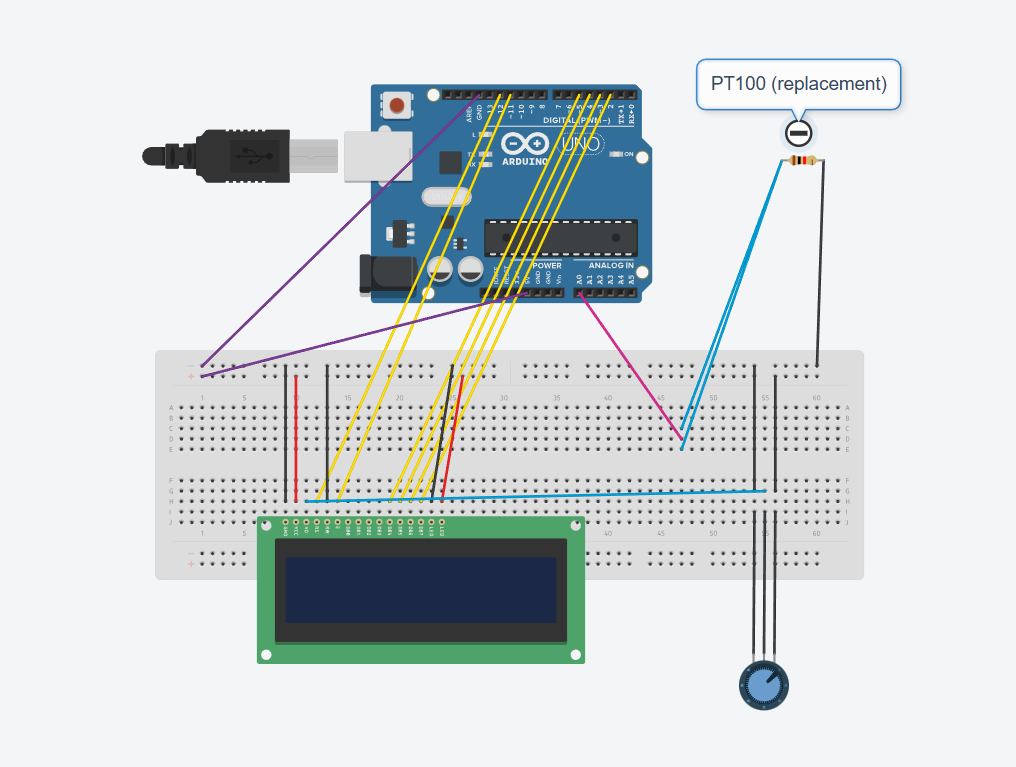
\includegraphics[width=0.8\linewidth]{image3.png}
    \caption{CIRCUIT DIAGRAM}
\end{figure}


\newpage
\section{USING LINEAR REGRESSION:}
Linear Regression Model for Calibration
The main formula used in calculating the temperature (using the PT100) is

\begin{equation}
    T \approx a_0 + [a_1 \cdot V] + [a_2 \cdot V^2]
\end{equation}
        
Now, based on the values of Voltages obtained and Temperatures of the surroundings, we are supposed to approximate the values of $a_0$, $a_1$ and $a_2$.
The equation {1} can be expressed in the form of a matrix equation
\begin{equation}
    A \cdot \textbf{x} = b
\end{equation}
 		
where $A =\begin{bmatrix}1 & T_1 & T_1^2 \\1 & T_2 & T_2^2 \\\vdots & \vdots & \vdots \\1 & T_n & T_n^2\end{bmatrix}$, $x = \begin{bmatrix}a_0\\a_1\\a_2\end{bmatrix}$ and $b = \begin{bmatrix}V_1 \\V_2 \\\vdots \\V_n\end{bmatrix}$

This equation can be solved using the \textbf{method of least squares} as mentioned in the question.\\
Since we need minimum error in finding the values of the constants in equation {1},
The residual $||Ax - b||^2$ should be minimum which means, $(Ax - b)\cdot(Ax - b)^T$ should be minimum on x.\\
Differentiating the equation and setting the gradient to zero,
\begin{equation}
    f(\textbf{x}) = ||A\textbf{x} - b||^2 = (A\textbf{x} - b)^T \cdot (A\textbf{x} - b).
\end{equation}

\begin{equation}
    d[f(\textbf{x})] / dx = 0
\end{equation}

\begin{equation}
    2 A^T\cdot A \cdot\textbf{x} - 2 A^T \cdot b = 0
\end{equation}

 \begin{equation}
     A^T\cdot A\cdot \textbf{x} = A^T \cdot b
 \end{equation}
From here,

\begin{equation}
    \textbf{x} = (A^T A)^{-1} \cdot A^T\cdot b 
\end{equation}
We can use this equation {7} to evaluate \textbf{x} in python for us.

\newpage

\section{EXPLANATION OF CODES USED:}

\begin{center}
    The python code used for calculating the matrix x
\end{center}
\begin{figure}[ht]
    \centering
    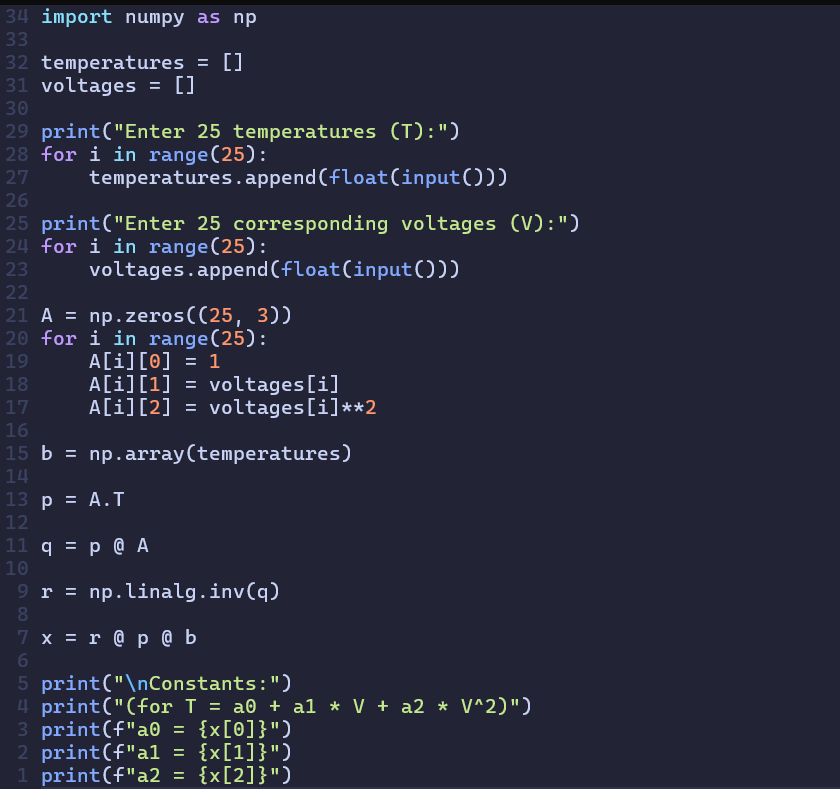
\includegraphics[width=0.8\linewidth]{image2.png}
    \caption{Least Square Method}
\end{figure}

The fairly simple code above defines a matrix A, x and b according to the notation above and prints the final approx. values of the constants.\\

It is just the creation of the matrices A and b which are later used in the evaluation of x.

\newpage

\begin{center}
    Before having the values of the constants
\end{center}
\begin{figure}[ht]
    \centering
    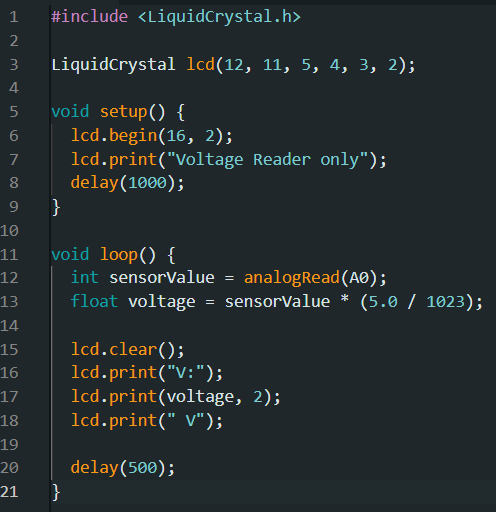
\includegraphics[width=0.6\linewidth]{image.png}
    \caption{Initial code in the Audrino IDE}
\end{figure}
It’s a simple code in C, which displays the voltage read by the “\textbf{A0} analog input”.\\
The multiplication factor of \textbf{5/1023.0} is used as the voltage reading from analog input is multiplied by 5/1023.0 to convert the raw \textbf{ADC} (Analog-to-Digital Converter) value to a real-world voltage level in volts. \\
As the The Arduino Uno ADC converts input voltages between 0V and 5V into digital values from 0 to 1023 (a 10-bit range).

\newpage

\begin{center}
    After gaining the constants
\end{center}

\begin{figure}
    \centering
    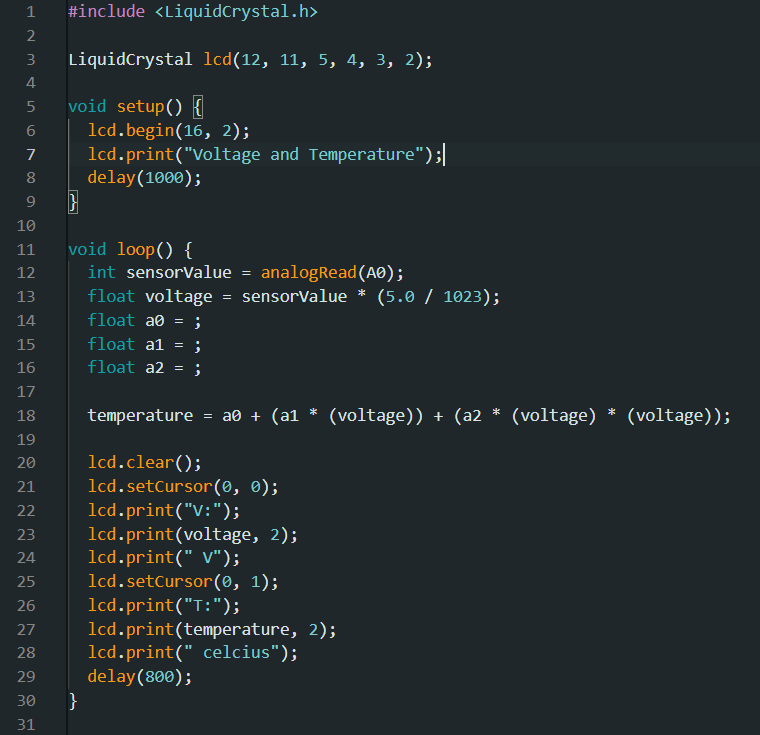
\includegraphics[width=0.5\linewidth]{image1.png}
    \caption{After gaining the values}
\end{figure}
It is just the previous code but with the addition of temperature variable which is calculated from the equation {1}.


\section{ERROR ANALYSIS:}

\begin{figure}[h]
    \centering
    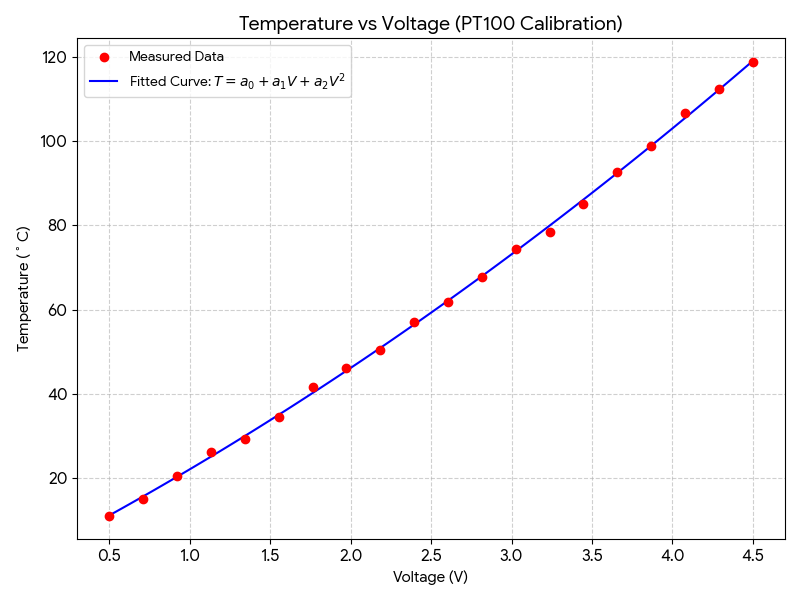
\includegraphics[width=0.6
    \linewidth]{Code_Generated_Image.png}
    \caption{Plot from matplotlib}
\end{figure}

The Mean Absolute Error (MAE): $\approx 1.07 °C$.\\
(Note : It is the average of all the errors obtained from the datapoints that we have.)\\

Also, another useful method of checking accuracy is coefficient\textbf{oefficient of determination} which is defined as
\begin{equation}
    R^2 = 1 - \frac{\text{Sum of squared errors}}{\text{Total sum of squares}}
\end{equation}

For our PT100 Thermometer model $R^2 \approx 0.975$. 

\section{CONCLUSION:}
Our Digital Thermometer made using a PT100 and a voltage divider is accurate and uses linear regression with the method of least squares to calculate the temperature as a function of voltage. \\
The final equation obtained by us is:
\begin{equation}
    T = (-7635.8621618788) + (5168.0892433551\cdot V) - (863.67569212067 \cdot V^2)
\end{equation}


\end{document}
